% a tikz figure for feature fusion block diagram

\usetikzlibrary{shapes}

\tikzstyle{data}=[draw,thick,rounded corners,minimum height=1.5cm,text width=2cm,align=center]
\tikzstyle{process}=[rectangle,draw,thick,minimum height=1.5cm,text width=2cm,align=center]

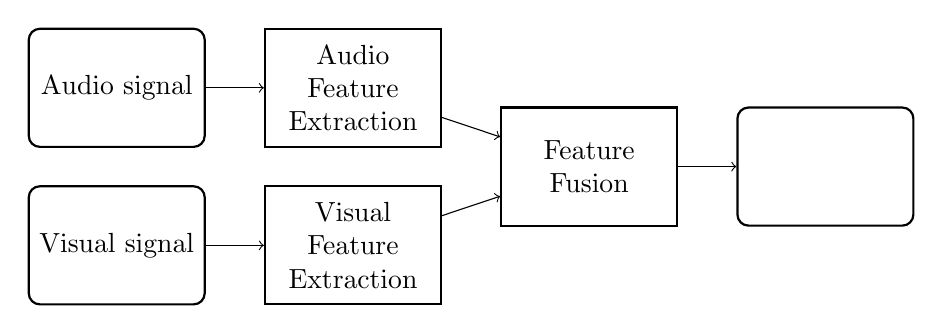
\begin{tikzpicture}[]
  \node[data] (iv) at (0,0) {Visual signal};
  \node[process] (pv) at (3,0) {Visual Feature Extraction}
    edge [<-] (iv);
  \node[data] (ia) at (0,2) {Audio signal};
  \node[process] (pa) at (3,2) {Audio Feature Extraction}
    edge [<-] (ia);
  \node[process] (ff) at (6,1) {Feature Fusion}
    edge [<-] (pv)
    edge [<-] (pa);
  \node[data] (o) at (9,1) {}
    edge [<-] (ff);
\end{tikzpicture}

